\chapter{Día 3}

\section{Animaciones Usando Sprites}

\subsection*{¿Cómo animar Sprites?}

Los componentes \component{SpriteImagen} son objetos especiales que
representan figuras que se mueven por la pantalla. A partir de ahora
los llamaremos simplemente \emph{sprites}. Los sprites están
especialmente diseñados para la creación de animaciones y videojuegos,
y deben utilizarse dentro de un componente \component{Lienzo}. Dentro
de un lienzo, el sprite tiene una \property{Dirección}, una
\property{Velocidad} y un \property{Intervalo}. Además, un sprite puede
colisionar con los bordes del lienzo, y con otros
sprites. La~\Cref{fig:spriteMap} cómo se orienta un sprite dentro del
lienzo. La dirección del sprite se representa mediante un ángulo,
entre 0 y 360 grados. El ángulo 0 representa el movimiento hacia la
derecha, y el ángulo 180 hacia la izquierda. Además, los bordes del
lienzo están identificados por números, como se ve en la figura.

\begin{figure}[H]
\centering
\includegraphics[scale=0.5]{spriteMap}
\caption{Configuración del \component{Lienzo} para la animación de Sprites.}
\label{fig:spriteMap}
\end{figure}

\paragraph{¿Cómo reduces la velocidad de un sprite, suavemente, a 100
  pixeles por segundo?}

La velocidad de un \component{SpriteImagen}, que se mide en pixeles
por segundo, es determinada por dos propiedades. La propiedad
\property{Intervalo} especifica cada cuantos milisegundos el sprite se
va a mover, y es muy similar a la propiedad
\component{Reloj.IntervaloDelTemporizador}. La propiedad
\property{Velocidad} específica cuántos pixeles el sprite se moverá en
cada intervalo. En el ejemplo que se muestra en la~\Cref{fig:Sprite1}
el sprite se mueve 5 pixeles cada 50 milisegundos, o 1 píxel cada 10
milisegundos---o sea, 100 pixeles/segundo.

\begin{figure}[H]
\centering
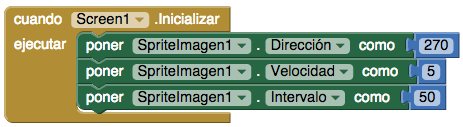
\includegraphics[scale=0.5]{Sprite1}
\caption{Ajustando la dirección, velocidad e intervalo de un sprite.}
\label{fig:Sprite1}
\end{figure}

La propiedad de \property{Dirección} del sprite especifica la
dirección en la cual se mueve. Como se ilustra en
la~\Cref{fig:Sprite1}, el sprite se moverá hacia abajo con una
orientación de 270 grados.

\paragraph{Ejemplo 2: ¿Cómo hacer rebotar una pelota?}

\AppInventor tiene un bloque \block{Botar} que provoca que una pelota
rebote en el borde del lienzo. Típicamente se usa \block{Botar} dentro
del controlador de eventos \block{Pelota.TocarBorde}, dado que este
controlador de eventos indica cual borde ha sido alcanzado, como
parámetro, por lo que puedes conectar este parámetro en la función
\block{Botar}---que necesita saber desde que borde rebotar.

También puedes hacer rebotar otros objetos (sprites o pelotas). El
controlador de eventos \block{EnColisiónCon} se activa cuando dos
objetos chocan. Sin embargo, la función \block{Botar} solamente
funciona en el borde de un lienzo, así que no puede usarse para
colisiones en general. Lo que sí puedes hacer es hacer rebotar el
sprite o pelota en la dirección opuesta a la que tenía antes de la
colisión, configurando su \property{Orientación} como 360 menos el
valor actual. Esto se ilustra en la~\Cref{fig:Sprite2}.

\begin{figure}[H]
\vspace{3em}
\centering
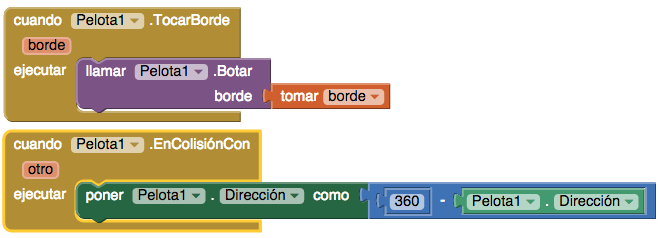
\includegraphics[scale=0.5]{Sprite2}
\caption{Programando una \component{Pelota} para que rebote al tocar
  el borde, y para que invierta su dirección al chocar con otro sprite
u objeto animado.}
\label{fig:Sprite2}
\end{figure}

\subsection*{Desafíos Animados}

\paragraph{Desafío 1: Animación Básica}

Para los siguientes desafíos, necesitarás un componente
\component{Lienzo} que ocupe todo lo ancho de la pantalla y que tenga
unos 300 pixeles de \property{Alto}.  Agrega un botón con texto
``Iniciar!'' abajo del lienzo. Crearás dos aplicaciones distintas:

\begin{enumerate}

\item Mover a la izquierda, abajo y en diagonal usando un
  \component{Reloj}.

  Agregar un componente \component{Reloj} y tres componentes
  \component{Pelota} en el \component{Lienzo}.  Cuando se hace click
  en el botón Iniciar las pelotas deben empezar a moverse dentro del
  lienzo (puedes obtener un movimiento suave al configurar el
  Intervalo de tiempo del \component{Reloj} en 50 milisegundos). Una
  pelota debería ir hacia abajo, otra a la izquierda y otra en
  diagonal. Las pelotas deben parar cuando tocan el borde del
  lienzo. Para este desafío usa sólo 1 componente \component{Reloj} y
  \emph{NO} uses las propiedades de animación internas del componente
  \component{Pelota} (velocidad etc.).

\item Mover a la izquierda, abajo y en diagonal usando una animación
  de Sprite.

  Para este desafío vas a repetir el comportamiento del punto anterior
  pero sin usar un componente \component{Reloj}. En vez de eso,
  utiliza las propiedades de animación internas del componente Pelota:
  \property{Velocidad}, \property{Intervalo} y \property{Dirección}.

\end{enumerate}

\paragraph{Discusión: Velocidad y Cuadros por Segundo}

\begin{enumerate}

\item ¿Qué tan rápido se estaban moviendo tus objetos en el ejercicio
anterior?

\item ¿Cómo determinar la velocidad de tus objetos cuando usas: a) una
  animación Sprite b) un contador de tiempo?. Indica una fórmula para
  cada caso.

\item Los Cuadros por Segundo (CPS) es una medición usada en películas
  y animaciones. Indica cuantas veces por segundo la película se
  actualiza.  ¿Qué CPS se necesita para que el cambio no sea notado
  por el ojo humano?  (Puedes buscarlo en Google)

\item ¿Cuál es el CPS de un juego si el
  \property{IntervaloDelTemporizador} es de 100 milisegundos.

\item Ejercicio de código: modifica uno de tus aplicaciones para que
  un objeto se mueva 50 pixeles por segundo y otro objeto se mueva a
  100 pixeles por segundo.

\end{enumerate}

\paragraph{Desafío 2: Ida y Vuelta }

Crea nuevas aplicaciones para los comportamientos siguientes:

\begin{enumerate}

\item Cuando se presiona un botón, una pelota hace idas y vueltas
  perpetuas en la pantalla.

  \begin{itemize}
  \item Hazlo sin un componente \component{Reloj} (o sea, con una
    animación de Sprite/Pelota).

  \item Hazlo con un componente \component{Reloj}.
  \end{itemize}

\item Cuando se presiona un botón, una pelota se mueve haciendo idas y
  vueltas perpetuas desde el borde izquierdo de la pantalla hasta la
  mitad de la pantalla.

  \begin{itemize}
  \item Hazlo sin un componente \component{Reloj} (o sea, con una
    animación de Sprite/Pelota).

  \item Hazlo con un componente \component{Reloj}.
  \end{itemize}

\end{enumerate}

\section{Tutorial: Pong}

En este tutorial aprenderás a programar una versión sencilla del
clásico juego \appName{Pong}. Hacer este juego te ayudará a
familiarizarte con la animación de sprites, a manejar colisiones, y a
definir procedimientos para que así puedas programar mejor!

A diferencia de los tutoriales anteriores, en este tutorial te
entregaremos un esqueleto de la aplicación, con la interfaz de usuario
ya desarrollada. Tu misión es programar los comportamientos de los
distintos elementos del juego.

La interfaz de usuario final para la aplicación se muestra en
la~\Cref{fig:Pong1}:

\begin{figure}[H]
\vspace{3em}
\centering
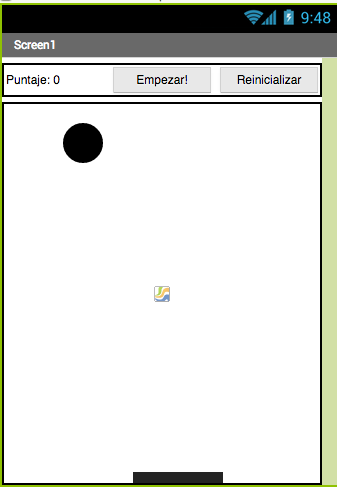
\includegraphics[scale=0.5]{Pong1}
\caption{Interfaz de usuario del juego \appName{Pong}}
\label{fig:Pong1}
\end{figure}

Para programar este juego debes seguir los siguientes pasos:

\begin{enumerate}

\item Programa una \component{Pelota} que se mueva en dirección hacia
  abajo. La pelota inicia su movimiento cuando se presiona el botón
  ``Empezar'' (\Cref{fig:Pong2}).

\begin{figure}[H]
\centering
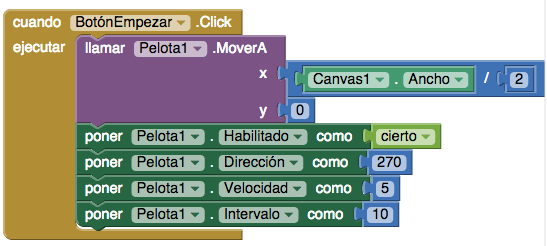
\includegraphics[scale=0.5]{Pong2}
\caption{La pelota se mueve hacia abajo cuando comienza el juego.}
\label{fig:Pong2}
\end{figure}

\item En el programa anterior la pelota es muy predecible, porque
  siempre va en línea recta hacia abajo desde el medio de la
  pantalla. Ahora programa la pelota para que baje en una dirección
  aleatoria---pero que aún es hacia abajo ¿Qué ángulos son ``hacia
  abajo''? (\Cref{fig:Pong3}).

\begin{figure}[H]
\centering
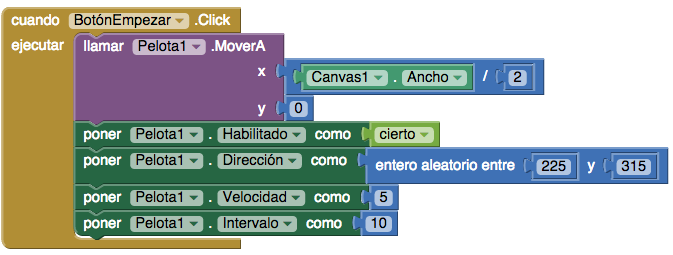
\includegraphics[scale=0.5]{Pong3}
\caption{La pelota se mueve hacia abajo en una dirección aleatoria.}
\label{fig:Pong3}
\end{figure}

\item Programa los rebotes de la pelota: contra los bordes y contra la
  barra.

\begin{figure}[H]
\centering
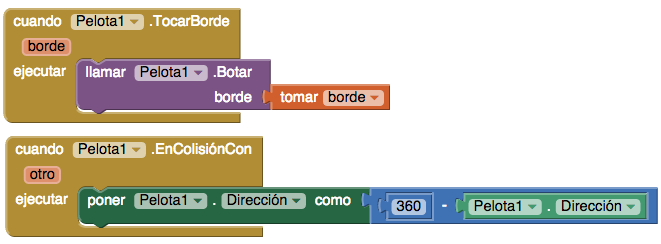
\includegraphics[scale=0.5]{Pong4}
\caption{La pelota rebota al tocar los bordes y al colisionar con la barra.}
\label{fig:Pong4}
\end{figure}

\item Programa la barra para que se mueva cuando el usuario arrastre
  el dedo. La barra sólo se mueve horizontalmente (o sea, sólo en la
  coordenada X) (\Cref{fig:Pong5}).

\begin{figure}[H]
\centering
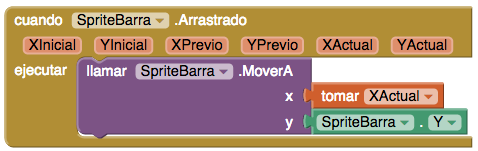
\includegraphics[scale=0.5]{Pong5}
\caption{La barra se mueve según el usuario arrastre el dedo sobre ella.}
\label{fig:Pong5}
\end{figure}

\item Modifica el programa para obtener 1 punto cada vez que la barra
  golpea la pelota. Para esto vas a usar un procedimiento con
  argumentos, averigua por ti mismo, o consulta a tu tutor al
  respecto (\Cref{fig:Pong6}).

\begin{figure}[H]
\centering
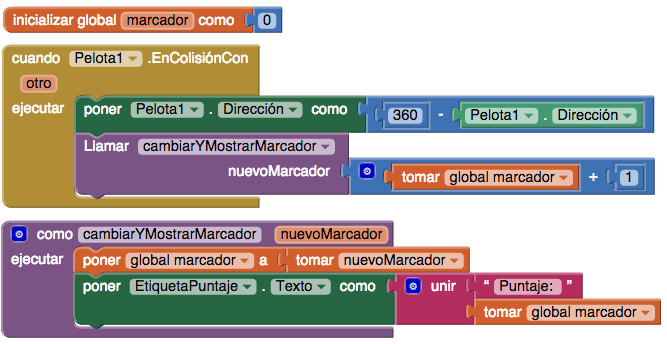
\includegraphics[scale=0.5]{Pong6}
\caption{Aumentando el puntaje cada vez que se golpea la pelota con la
barra.}
\label{fig:Pong6}
\end{figure}

\item Modifica el programa para que el juego termine si la pelota
  choca con el borde de abajo (\Cref{fig:Pong7}).

\begin{figure}[H]
\centering
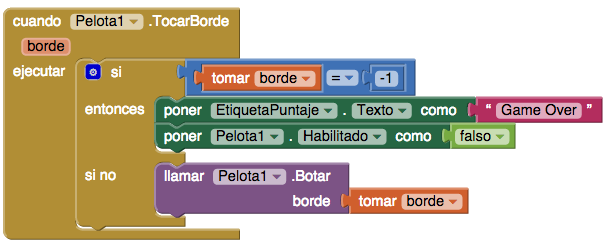
\includegraphics[scale=0.5]{Pong7}
\caption{El juego termina cuando la pelota choca con el borde de abajo.}
\label{fig:Pong7}
\end{figure}

\item Agrega un componente \component{Sonido} y modifica el programa para agregar distintos efectos de sonido
  cuando la pelota choca en la barra, toca los bordes, y para el fin
  del juego (los archivos ya vienen incorporados en el proyecto
  inicial, ver~\Cref{fig:Pong8}).

\begin{figure}[H]
\vspace{3em}
\centering
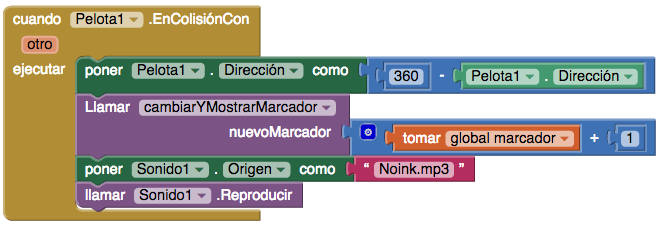
\includegraphics[scale=0.5]{Pong8}
\caption{Efectos de sonido para las colisiones, toque de bordes y fin
  del juego.}
\label{fig:Pong8}
\end{figure}

\item Agrega un component \component{CasillaDeVerificación} para que
  el usuario puede apagar/prender el sonido (\Cref{fig:Pong9}).

\begin{figure}[H]
\centering
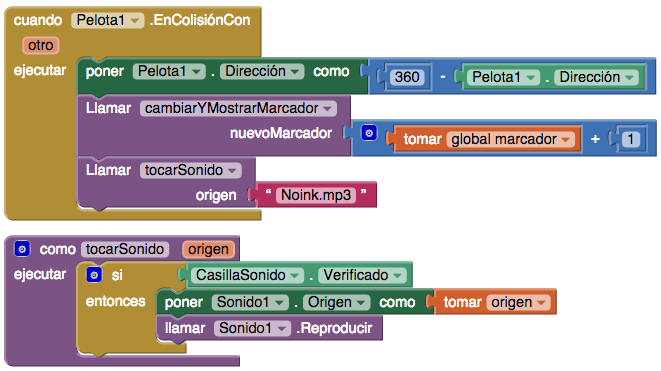
\includegraphics[scale=0.5]{Pong9}
\caption{La reproducción de sonidos depende del valor de la casilla de
verificación.}
\label{fig:Pong9}
\end{figure}





\end{enumerate}

\section{Proyecto: Crea tu Propio Juego o Aplicación}

Crea una aplicación con animaciones similares--pero más
complejas---que en el juego \appName{Atrapa el Topo} y \appName{Pong}.

La aplicación debe tener las siguientes funcionalidades:

\begin{itemize}

\item Objetos que se mueven en el tiempo (por ejemplo una nave
  espacial que atraviesa la pantalla).

\item Objetos que se mueven o son transformados en reacción a la
  actividad del usuario (por ejemplo el sensor de orientación para
  controlar el movimiento).

\item Objetos que aparecen o desaparecen en reacción a las actividades
  del usuario (por ejemplo, un asteoride que desaparece cuando recibe
  un disparo).

\item Uso de bloques condicionales.

\item Uso de bloques \block{EnColisiónCon} y \block{TocarBorde}.

\end{itemize}

¡Se creativo! No necesitas crear un juego, puedes crear lo que tu
quieras mientras muestre todos los comportamientos listados arriba.
Comparte tu idea con tu tutor y aseguráte que tienes todos los
comportamientos requeridos.

\section{Material de Apoyo: Variables, o Cómo Programar la Memoria de
tu Aplicación}

Así como las personas necesitan recordar cosas, también las
aplicaciones lo necesitan. En este material de apoyo volveremos al
tema de las variables, pero ahora con mayor profundidad y
detalle. Como vimos anteriormente, la idea esencial de usar variables
es programar una aplicación para que recuerde información.

Cuando alguien te dice el número de teléfono de una pizzería, tu
cerebro lo almacena en una \emph{celda de memoria}. Si alguien
menciona algunos números para que tú los sumes, tú también almacenas
estos números y los resultados intermedios en una celda de memoria. En
estos casos, no estás totalmente conciente de cómo tu cerebro almacena
o recuerda la información.

Una aplicación también tiene memoria, pero su funcionamiento interno
es mucho menos misterioso que el de tu cerebro. Ahora veremos en
detalle cómo manejar la memoria de una aplicación, cómo almacenar
información en ella, y cómo recuperar esa información en un momento
posterior.

\subsection*{Celdas de Memorias Definidas}

La memoria de una aplicación consiste de una serie de celdas de
memoria definidas. Algunas de estas celdas de memoria se crean cuando
arrastras un componente en tu aplicación. Estas celdas (o espacios
abiertos) se llaman \emph{propiedades}. También puedes definir celdas
de memoria definidas que no sean asociadas con un componente
específico. Estas se llaman \emph{variables}. Aunque las propiedades
están típicamente asociadas a lo que es visible en la app, las
variables pueden ser asociadas a la \emph{memoria escondida} de la
aplicación.

\subsection*{Propiedades}

Tú, como usuario de una aplicación, puedes ver componentes visibles
como botones, cuadros de texto y etiquetas. Pero adentro, cada
componente es completamente definido por una serie de propiedades. Los
valores almacenados en la memoria de cada propiedad determina cómo
aparece el componente. Tú configuras los valores de las propiedades
directamente en el Diseñador de Componentes. Por ejemplo,
la~\Cref{fig:Variable1} muestra el panel para modificar las
propiedades de un componente \component{Lienzo}.

\begin{figure}[H]
\centering
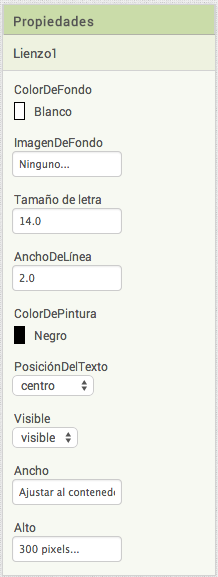
\includegraphics[scale=0.5]{Variable1}
\caption{Hoja de propiedades para un componente lienzo.}
\label{fig:Variable1}
\end{figure}

El componente \component{Lienzo} tiene varias propiedades de distintos
tipos. Por ejemplo el \property{ColorDeFondo} y el
\property{ColorDePintura} son celdas de memoria que contienen un
color. La propiedad \property{ImagenDeFondo} contiene un nombre de
archivo (como \mediafile{gatito.png}).

La propiedad \property{Visible} contiene un valor booleano (verdadero
o falso, dependiendo si se selecciona la opción o no). El
\property{Ancho} y \property{Alto} contienen un número o una
designación especial (por ejemplo, ``Ajustar al Contenedor'').

Cuando configuras una propiedad en el \componentDesigner, especificas
el valor inicial de está propiedad, o sea su valor cuando se inicia la
aplicación. Los valores de las propiedades también pueden ser
modificados cuando la aplicación se ejecuta, mediante el uso de
bloques. Pero, al cambiar los valores durante la ejecución, los
valores que aparecen en el \componentDesigner no cambian---estas
propiedades siempre muestran solamente los valores iniciales. Esto
puede confundir cuando pruebas una aplicación, pues el valor actual de
las propiedades de la aplicación cuando se ejecuta no son visibles.

\subsection*{Definir Variables}

Al igual que las propiedades, las variables son celdas de memoria,
pero que no están asociadas a un componente en particular. Se define
una variable cuando necesitas que tu aplicación guarde algo en memoria
que no haya sido guardado ya en una propiedad de un componente. Por
ejemplo, puede ser que un juego tenga que recordar el nivel alcanzado
por el usuario. Si el número del nivel apareciera en un componente
\component{Etiqueta}, no necesitarías una variable, porque podrías
simplemente almacenar el nivel en la propiedad de \property{Texto} de
la etiqueta. Pero si el número de nivel no es algo que será visible
por el usuario, necesitas definir una variable para guardar esta
información.

Otra diferencia es que mientras que las propiedades se crean automáticamente cuando arrastras un
componente en el \designer, las variables se definen explícitamente en el
\blockEditor al arrastrar un bloque ``inicializar global nombre''. Puedes nombrar la variable al hacer click en el texto que
dice ``nombre'' dentro del bloque, y puedes especificar un valor inicial
al arrastrar un bloque (número, texto, color, lista) y conectarlo al
bloque de inicialización. Por ejemplo, para crear una variable llamada ``marcador'' con un valor inicial de
0, sigue los siguientes pasos, que se muestran en la~\Cref{fig:Variable2}:

\begin{enumerate}

\item Arrastra el bloque  ``inicializar global nombre'' desde la sección
  ``Variables'' hacia el espacio de trabajo.

\item Cambia el nombre de la variable al hacer click en el texto
  ``nombre'' y escribe ``marcador''.

\item Configura el valor inicial de la variable al arrastrar un bloque
  numérico, con valor 0, y conectarlo con la definición de la
  variable.

\begin{figure}[H]
\centering
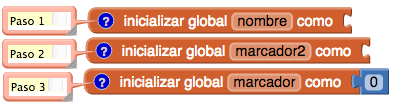
\includegraphics[scale=0.5]{Variable2}
\caption{Inicializando la variable global \variable{marcador} con
  valor 0.}
\label{fig:Variable2}
\end{figure}

\end{enumerate}

Cuando defines una variable, pides a la aplicación crear una celda de
memoria para guardar un valor. Estas celdas de memoria, como las
propiedades, no son visibles por el usuario cuando funciona la
aplicación.

El bloque de inicialización que conectas en la declaración de la
variable especifica el valor que estará en la celda cuando se inicia
la aplicación. A parte de inicializar con números o texto, también
puedes inicializar la variable con un bloque \block{crear una lista
  vacía} o \block{construye una lista}. Esto indica a la aplicación
que la variable guardará un listado de celdas de memoria en lugar de
un solo valor. Trabajaremos con listas en el Día 4 del taller.

\subsection*{``Poner'' y ``Tomar'' una Variable}

Cuando defines una variable, \AppInventor crea dos bloques para ella,
un bloque \block{poner} y un bloque \block{tomar}. Puedes acceder a
estos bloques al pasar el mouse por encima del nombre de la variable
en el bloque de inicialización, como se ve en la~\Cref{fig:Variable3}.

\begin{figure}[H]
\centering
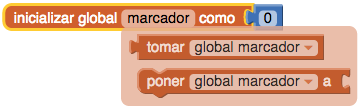
\includegraphics[scale=0.5]{Variable3}
\caption{El bloque de inicialización contiene bloques de configurar y
  obtener para esta variable.}
\label{fig:Variable3}
\end{figure}

El bloque \block{poner global marcador} te permite modificar el valor
almacenado en la variable. Por ejemplo, los bloques de
la~\Cref{fig:Variable4} indican un 5 en la variable
\variable{marcador}. El término \emph{global} en el bloque se refiere
al hecho de que la variable puede ser usada en todos los controladores
de eventos y procedimientos del programa. La nueva versión de
\AppInventor permite también definir variables \emph{locales}, que son
específicas a un controlador de eventos o a un procedimiento
específico.

\begin{figure}[H]
\centering
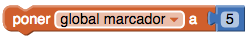
\includegraphics[scale=0.5]{Variable4}
\caption{Poner un número 5 en la variable marcador.}
\label{fig:Variable4}
\end{figure}

El bloque \block{tomar global marcador} permite obtener o rescatar el valor
de una variable. Por ejemplo, si quieres chequear si el valor dentro de
la celda de memoria era superior a 100, tienes que conectar el bloque
\block{tomar global marcador} en un bloque condicional, tal como se
muestra en la~\Cref{fig:Variable5}.

\begin{figure}[H]
\centering
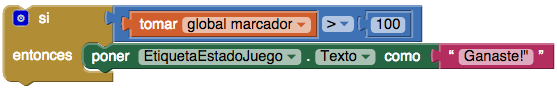
\includegraphics[scale=0.5]{Variable5}
\caption{Usando el bloque marcador global para obtener el valor
  almacenado en la variable.}
\label{fig:Variable5}
\end{figure}

\subsection*{Configurar una Variable como Expresión}

En las variables puedes poner valores simples, como 5, pero
frecuentemente configurarás la variable como una \emph{expresión} más
compleja (\emph{expresión} es el término informático que se le da a
una fórmula o cálculo). Por ejemplo, cuando alguien pierda 10 puntos
en un juego, necesitas modificar la variable \variable{marcador} como
``10 menos que su valor actual''. Otro ejemplo es en un juego como
\appName{Atrapa el Topo}, cambias la ubicación horizontal (x) del topo
a una ubicación aleatoria dentro del lienzo. Tanto los valores simples
como las expresiones complejas se conectan al argumento del bloque
\block{poner global}.

\subsection*{Incrementar una Variable}

Tal vez la expresión más común es para \emph{incrementar una
  variable}, o configurar una variable basado en su propio valor
actual. Por ejemplo, en un juego, cuando el jugador marca un punto, la
variable \variable{marcador} puede ser incrementada en 5
puntos. La~\Cref{fig:Variable6} ilustra los bloques que hay que usar
para programar este comportamiento.

\begin{figure}[H]
\vspace{3em}
\centering
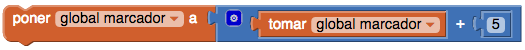
\includegraphics[scale=0.5]{Variable6}
\caption{Se incrementa la variable \variable{marcador} en 5 puntos.}
\label{fig:Variable6}
\end{figure}

Si puedes entender este tipo de bloques, vas bien encaminado para
convertirte en un programador!

Estos bloques se leen de la siguiente manera: ``configurar el marcador
como 5 veces más que su valor actual'', que es una manera para decir,
\emph{incrementa} la variable en 5. El código funciona de la siguiente
manera: los bloques se leen de adentro hacia afuera---no de izquierda
a derecha.  Entonces se lee primero el bloque ``tomar global
marcador'' y el número 5. Luego el bloque de suma es ejecutado y el
resultado se pone en la variable \variable{marcador}.

Suponiendo que hubiera un 10 en la celda de memoria para
\variable{marcador} antes de ejecutar estos bloques, la aplicación
ejecutaría los siguientes pasos:

\begin{enumerate}

\item Obtener el 10 de la celda de memoria \variable{marcador},
  mediante la evaluación del bloque \block{tomar}.

\item Sumar 5 con el 10 obtenido, para obtener 15.
\item Poner el resultado, 15, en la celda de memoria
  \variable{marcador}, mediante la evaluación del bloque
  \block{poner}.
\end{enumerate}

\subsection*{Construir expresiones complejas}

En la sección ``Matemáticas'' del \blockEditor, \AppInventor provee un amplio conjunto de funciones matemáticas
similares a las que podrás encontrar en una planilla de Excel o en una
calculadora. La~\Cref{fig:Variable7} muestra estas funciones.

\begin{figure}[H]
\vspace{3em}
\centering
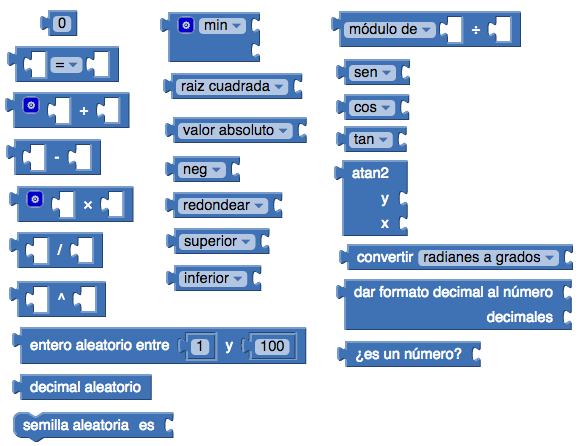
\includegraphics[scale=0.5]{Variable7}
\caption{Los bloques contenidos en la sección ``Matemáticas''.}
\label{fig:Variable7}
\end{figure}

Puedes usar estos bloques para construir una expresión compleja y
conectarla en el \emph{lado derecho} de un bloque \block{poner
  global}.  Por ejemplo, para mover un sprite a una columna aleatoria
dentro de los bordes de un lienzo, tienes que configurar una expresión
que consiste de una multiplicación, una resta, una propiedad
\property{Lienzo.Ancho}, una propiedad \property{SpriteImagen.Ancho} y
un bloque \block{entero aleatorio}, como se muestra en
la~\Cref{fig:Variable8}.

\begin{figure}[H]
\centering
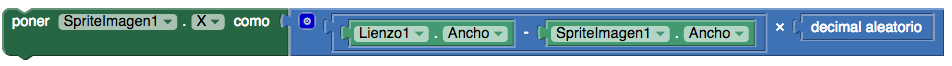
\includegraphics[scale=0.5]{Variable8}
\caption{Puedes usar bloques de ``Matemáticas'' para construir expresiones complejas.}
\label{fig:Variable8}
\end{figure}

Al igual que el ejemplo anterior sobre cómo incrementar una variable, los bloques
se leen desde adentro hacia afuera. Suponiendo que el
\component{Lienzo} tiene un \property{Ancho} de 300 pixeles y el
\component{SpriteImagen} tiene un \property{Ancho} de 50 pixeles, la aplicación
ejecutaría los siguientes pasos:

\begin{enumerate}

\item Obtener el 300 y el 50 de las celdas de memoria para
  \property{Lienzo1.Ancho} y \property{SpriteImagen1.Ancho},
  respectivamente.
\item Restar: $300 -- 50 = 250$.
\item Llamar a la función \block{entero aleatorio} para obtener un
  número entre 0 y 1 (por ejemplo 0,5).
\item Multiplicar: $250 * 0.5 = 125$.
\item Poner el 125 en la celda de memoria para la propiedad
  \property{X} de \component{SpriteImagen1}.
\end{enumerate}

\subsection*{Mostrar las Variables}

Cuando modificas la propiedad de un componente, como en el ejemplo
previo, la interfaz de usuario se modifica directamente. Esto no es
cierto para las variables: cambiar una variable no tiene efecto
directo en la apariencia de la aplicación. Si solamente incrementaste
una variable \variable{marcador} pero no modificaste la interfaz de
usuario de alguna otra manera, el usuario no podrá saber que hubo un
cambio. Es como un árbol que se cae en el bosque: si nadie estuvo para
escucharlo, ¿ocurrió de verdad?

A veces no quieres que se manifieste el cambio en la interfaz de
usuario cuando cambia una variable. Por ejemplo, en un juego puedes
hacer un seguimiento estadístico (tiros fallidos) que solamente
aparecerá al terminar el juego.

Esta es una de las ventajas de guardar datos en una variable, en
comparación con la propiedad de un componente: te permite mostrar los
datos que quieres en el momento que elijas. También te permite separar
la parte computacional de tu aplicación de la interfaz de usuario,
facilitando cambios posteriores de dicha interfaz.

Por ejemplo, en un juego podrías guardar el marcador directamente en
una \component{Etiqueta} o en una variable. Si lo guardas en una
etiqueta, tienes que incrementar las propiedades de texto de la
etiqueta cuando se marcan puntos, y el usuario verá los cambios
directamente. Si guardaste el marcador en una variable y se incrementa
la variable cada vez que se marcan puntos, tendrías que incluir
bloques para también escribir el valor de la variable en una etiqueta.

Sin embargo, si decidieras cambiar la aplicación para mostrar el
marcador de una manera distinta, por ejemplo con una barra de color,
la opción de una variable sería más fácil de cambiar. No necesitarías
modificar todos los lugares donde aparece el marcador sino que
solamente tendrías que modificar los bloques que muestran el marcador.

\subsection*{Variables locales}

Hasta el momento hemos hablado de variables \emph{globales} que se
definen con un bloque \block{inicializar global}. \emph{Global} se
refiere al hecho que la variable se puede usar en todos los
procedimientos y controladores de eventos de la
aplicación. \AppInventor también te permite definir variables
\emph{locales}, es decir, variables cuyo uso es restringido a un solo
controlador de eventos o procedimiento, como se muestra en
la~\Cref{fig:Variable9}.

\begin{figure}[H]
\centering
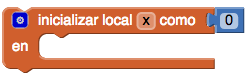
\includegraphics[scale=0.5]{Variable9}
\caption{Puedes definir una variable de alcance restringido (local).}
\label{fig:Variable9}
\end{figure}

Si la variable es requerida en un sólo lugar, es una buena idea
definirla como local en vez de global. Al proceder de tal manera,
limitas las dependencias en tu aplicación y te aseguras de que no
modificarás una variable por error. Imagina que una variable local es
como tu memoria privada en tu cerebro---no quieres que otros cerebros
puedan tener acceso a ella!

\subsection*{Resumen}

Cuando inicias una aplicación, ésta empieza a ejecutar sus operaciones
y a responder a eventos que ocurren. Al responder a eventos, la
aplicación a veces necesita recordar cosas. Para un juego, puede ser
que tenga que recordar el marcador de cada jugador o la dirección en
la cual se mueve un objeto.

Tu aplicación recuerda cosas con propiedades de componentes, pero
cuando necesitas memoria adicional no asociada a un componente, puedes
definir variables. Puedes almacenar valores dentro de una variable y
recuperar el valor actual, de la misma manera que con las
propiedades. Como los valores de propiedades, los valores variables no
son visibles para el usuario final. Si quieres que el usuario final
vea la información almacenada en una variable, agregas bloques que
muestran esta información en una etiqueta u otro componente de la
interfaz de usuario.
